% Chapter Template

\chapter{Long Range Communication Architecture} % Main chapter title

\label{Chapter3} % Change X to a consecutive number; for referencing this chapter elsewhere, use \ref{ChapterX}

\lhead{Chapter 3. \emph{Long Range Communication}} % Change X to a consecutive number; this is for the header on each page - perhaps a shortened title

In this chapter, we shall look at the long range communication architecture, menat for communication between ground station and the UAVs, and how it is integrated with the mesh network and ROS.

\section{Hardware}
Among the existing solutions for long range communication, radios based on 900Mhz spectrum seem popular. Compared to 2.4Ghz radios, there are a few reasons for this. First, the path loss for 2.4Ghz radios is higher than that of 900Mhz radios, reducing the received signal strength significantly over long distances. With the use of high gain directional antennas, the gap in the received signal strength between the radios of two spectra, can be eliminated, or even reversed. While this makes the 2.4Ghz radios favorable than 900Mhz radios in static point-to-point links, 900Mhz radios still have a much longer range than 2.4Ghz radios. Second, the 2.4Ghz spectrum is more vulnerable to the issues of penetration and blockages in the face of obstacles, while 900Mhz is more robust to them.

Note that much of 2.4Ghz hardware consists of wifi based solutions, based on the 802.11 hardware, and 802.11 was designed to be indoor, with short range, but high bandwidth. Consequently, hardware based on 802.11 is inefficient for use over long distances. While there are implementations of custom protocol stacks, instead of 802.11, on 2.4Ghz spectrum, these are almost always propietary and consequently, the modules are quite expensive. Considering all things, 900Mhz radios are still offer quite a promising solution for communication over long distances. One downside is that the 900Mhz radios typically offer lower bandwidth on the order of a few 100 Kbps, compared to 2.4Ghz solutions. Nonetheless, this should not be a problem as long as not too much data is demanded at the ground station, which is true in most applications.

\subsection{RFD900X}
RFD900X is third in line of popular 900Mhz radios by the company, RFDesign, the first two being RFD900 and RFD900+. The radio operates on frequency range 902-928 Mhz. It allows selectable transmit power upto 30dBm, in steps of 1dBm. It supports multiple air data rates from 4Kbps to 500Kbps. It has a UART interface supporting multiple baud rates from 9600 to 1000000. It has an advertised range of more than 50Kms in line of sight conditions, depending on antennas. The radios support a set of AT commands for configuring different parameters. There is decent documentation regarding the radios that can be found at \url{http://files.rfdesign.com.au/docs/}.

\begin{figure}[h]
	\centering
	\begin{subfigure}{0.5\textwidth}
		\centering
		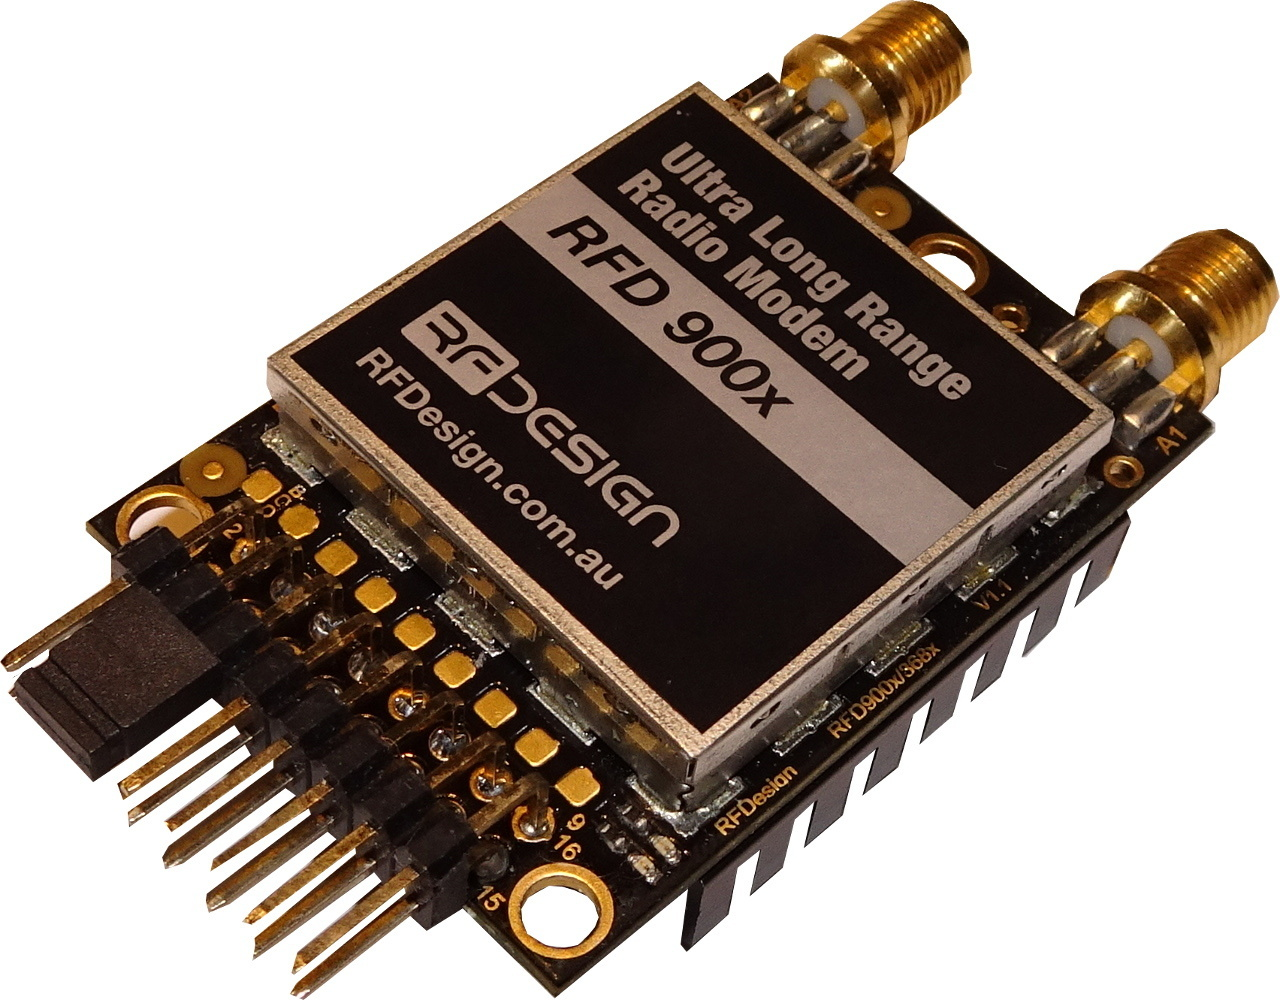
\includegraphics[scale=0.1]{Pictures/rfd1.jpg}
	\end{subfigure}%
	\begin{subfigure}{0.5\textwidth}
		\centering
		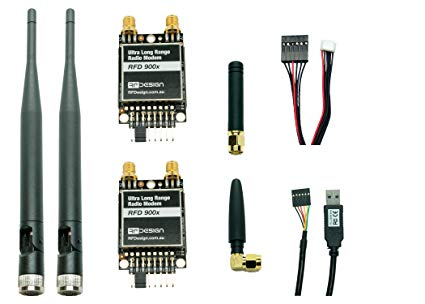
\includegraphics[scale=0.5]{Pictures/rfd2.jpg}
	\end{subfigure}
	\caption{RFD900x along with antennas and FTDI cables}
	\label{fig: rfd900x}
\end{figure}

The radios come with a default peer to peer firmware, which means that the radios can only be used in pairs. There are two other firmwares that can be flashed on radios, synchronous mesh and asynchronous mesh, which are point to multipoint firmwares. These firmwares can be flashed by a gui program called 'Modem Tools' that can downloaded from \url{http://files.rfdesign.com.au/}.

\subsubsection{Peer to Peer Firmware}
As mentioned, the radios come flashed with the peer to peer firmware by default. We may need to configure the radios with some parameters via the AT commands. For instance, the parameters NETID, SERIAL\_SPEED, AIR\_SPEED should be same on both the modems, among other things. Radios with same NETID can talk to each other. Essentially, any raw bytes input to the serial UART interface at one radio can be received at the serial interface of the other radio. Different pairs of radios with different NETIDs can only send and receive data to and from the radio with the same NETID. Even though you can have multiple pairs of radios wiht different NETIDs, as the total number of radios increase, interference also increases, increasing the errors in transmitted bytes.

\begin{figure}[h]
	\centering
	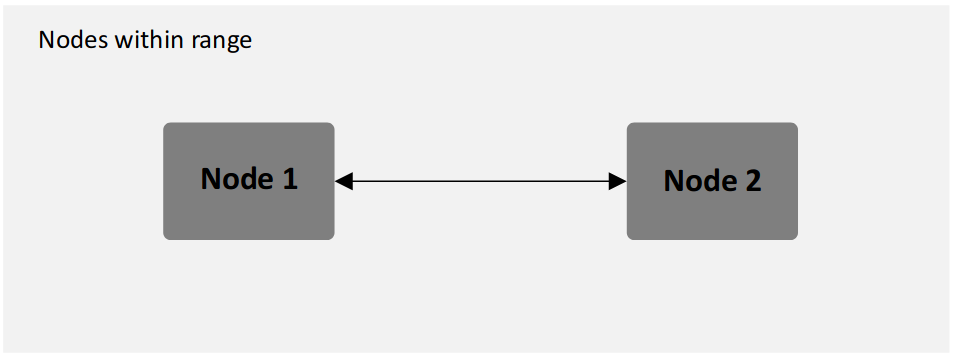
\includegraphics[scale=0.4]{Pictures/peer.png}
	\caption{modems in peer to peer configuration}
	\label{fig: rfdpeer}
	\captionsetup{font={footnotesize,bf,it}}
	\caption*{source: http://files.rfdesign.com.au/Files/documents/RFD900x\%20DataSheet\%20V1.1.pdf}
\end{figure}

\subsubsection{Synchronous Mesh Firmware}
While the peer to peer firmware allows communication only between a pair of radios, the asynchronous firmware is a point to multipoint firmware. Apart from the NETID parameter, there is a NODEID parameter, NODEDESTINATION parameter, NETCOUNT parameter among others, that can be set by the AT commands. Unlike the peer to peer firmware, more than two radios can have the same NETID. While using the synchronous firmware, one of the radios needs to be as a base node. This can be done by setting the NETID parameter to 0 and NODEID parameter to 1 on the base radio. We should also specify the number of radios with the parameter NETCOUNT. Each radio should be assigned a unique NODEID, from 1 to 15. By, specifying the NODEDESTINATION, the radio transmits the data to that node. If the NODEDESTINATION is set as 255, it enables broadcast mode and transmits to all the nodes.

In this configuration, the base radio assigns time slots to each of the other radios to communicate. Essentially, each radio transmits data only during its assigned time slot. So, even if other radios are not transmitting data, a radio waits for its time slot to transmit its data. This is inefficient when either not many radios are transmitting or they are not transmitting too often.

\begin{figure}[h]
	\centering
	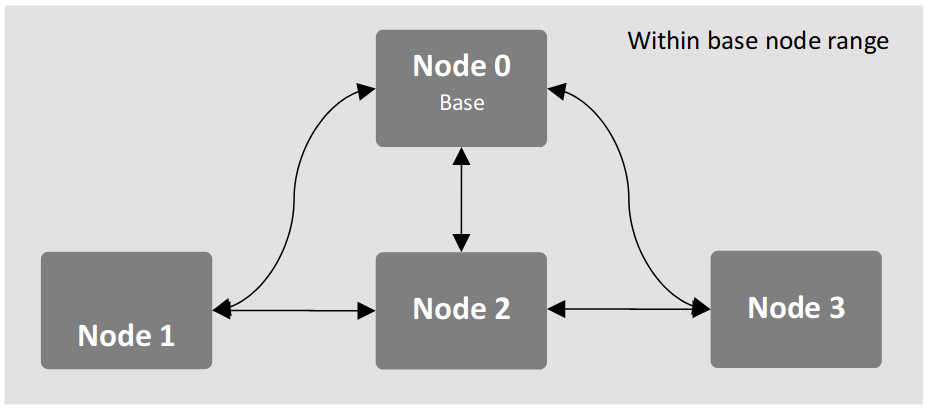
\includegraphics[scale=0.4]{Pictures/sync.png}
	\caption{modems in synchronous mesh configuration}
	\label{fig: rfdsync}
	\captionsetup{font={footnotesize,bf,it}}
	\caption*{source: http://files.rfdesign.com.au/Files/documents/RFD900x\%20DataSheet\%20V1.1.pdf}
\end{figure}

\subsubsection{Asynchronous Mesh Firmware}
Like synchronous firmware, this a point to multipoint firmware. But, in its configurable parameters, there is no NETCOUNT pararmeter, and instead of NODEDESTATION, there is a DESTID parameter. Here, the NODEID can be set to any unique value between 1 to 32767. The radio transmits to a receiver radio, specified by setting the parameter DESTID to the NODEID of the receiver radio. If the DESTID parameter is set as 65535, broadcast mode is enabled and the radio transmits to all the radios in the network.

While, in the synchronous firmware, each radio in the network, is assigned a time slot, for transmitting data, coordinated by the base radio, in the case of asynchronous firmware, there is no base radio which assigns time slots and the radios can transmit any time, asynchronously. If two radios transmit simultaneously and a packet collision happens, the radios retry to transmit the packet, multiple times, based on the parameter, MAX\_RETRIES.

\begin{figure}[h]
	\centering
	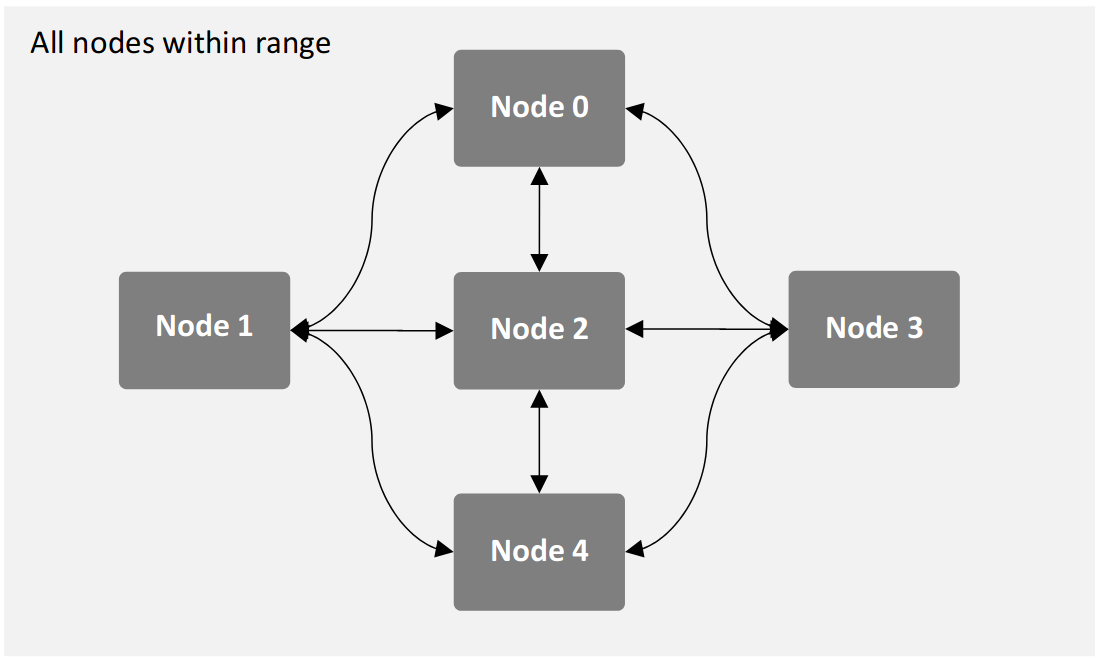
\includegraphics[scale=0.4]{Pictures/async.png}
	\caption{modems in asynchronous mesh configuration}
	\label{fig: rfdsync}
	\captionsetup{font={footnotesize,bf,it}}
	\caption*{source: http://files.rfdesign.com.au/Files/documents/RFD900x\%20DataSheet\%20V1.1.pdf}
\end{figure}

\section{Architecture and Integration with ROS}
Let us give a brief outline of the entire architecture, along with wifi mesh and the RFDs. As we described in the last chapter, the wifi routers connected to the host machines, will establish a mesh network among the host machines, which are running ROS. Thus, ros topics and services of any host machine can be acessed in any other host machine, as required. Now, the assumption is that, while the mesh network enables communication among the host machines, which are mounted on the UAVs, the communication between the UAVs and the ground station cannot be acheived by the mesh network as the ground station may be far away and out of range of the mesh. This is where the RFDs come in.

However, RFDs have a few downsides. First, they offer much lower data rate, which means that the data that is being sent down by the 
UAVs to the ground has to be minimal. Second, if all the UAVs are simultaneously transmitting data to the ground station, it would overwhelm the system in one way, or the other. This motivated us to come up with an architecture, where not all the UAVs are transmitting data down to the ground station, at any given time. We designate one of the UAVs as a leader, in the sense that it is the only UAV, that sends data down to the ground station. The leader, itself takes care of all the data, of the remaining UAVs as well, that needs to be sent to the ground station. This is possible since the leader has access to the data of all the remaining UAVs, as they are all connected via the mesh network.

One of the key assumptions is that all the UAVs are always connected via the mesh network, allowing the leader to access their data, as required. But, it may happen that some of the UAVs are out of range of the mesh network and are not accessible by the leader, or the leader itself, may come out of range, disconnecting it with the rest of the UAVs. This prompted us to extend the proposed architecture to address these problems.

In the coming sections, we propose and describe two architectures. First one is a \textit{Static Leader} architecture, where there is only one fixed leader, in the network. Clearly, this assumes that all the other UAVs are accessible by the leader via the mesh network. The second architecture, which we call \textit{Dynamic Leader} architecture is an extension of the first one, designed to address the shortcomings of the second one.

Before proceeding further, let us look at how ROS fits into the architecture, and the interfaces we have had to write for ROS.

\subsection{ROS}
ROS, running on the host machines of the UAVs, communicates with the onboard autopilot, which is connected to various sensors, and publishes all the sensor data and the state of the UAVs, on various ros topics. It also makes various ros services available, which upon calling would call corresponding services on the autopilot. Our aim was to make all the required data of all the UAVs available at the ground station, as ros topics and services.

Since the RFDs are serial radios and do not have a TCP/IP protocol stack, these radios cannot be integrated into ROS, as easily as the wifi mesh network. The reason for this is that, while ROS allows access of ros topics and services via TCP/IP, it does not have a serial interface. By serial interface, we mean the access of ros topics and services via a serial communication link. This has led us write our own serial interface for ROS. We have written this interface as an independent open source ROS node in a package, that anyone can use in their own applications. Both the node and the package are called \textit{serialros}.

\subsubsection{serialros}

\begin{figure}[h]
	\centering
	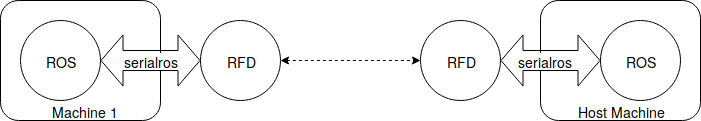
\includegraphics[scale=0.5]{Pictures/serialros.png}
	\caption{serialros, a serial interface to ROS}
	\label{fig: serialros}
	\captionsetup{font={footnotesize,bf,it}}
\end{figure}

The \textit{serialros} package allows sending and receiving of arbitrary ros topics via a serial communication link. It also allows access of ros services via a serial link. The node, when launched, monitors the serial port as specified and publishes any incoming messages, on their corresponding topics in the local machine. However, it does not transmit any ros messages of any topics, that are published on the local machine, via the serial port. For transmitting messages, from a topic that is being published on the local machine, via the serial port, the topic has to be specified in a configuration file. Similarly the services of a remote machine that we want to access on the local machine needs to be specified in the configuration file.

The package has a launch file \textit{serialros.launch}, that can be launched with \textit{roslaunch}, which launches the relevant nodes and starts publishing any incoming ros topics on the serial port, transmits any specified ros topics from the local machine and makes specified services from remote machines accessible in the local machine. The source code and instructions on how to use the package can be found at \url{https://github.com/saiadityachundi/serialros.git}.

\subsection{Static Leader}
In this architecture, we designate one of the UAVs as a leader. We assume that all the UAVs are always connected via the mesh network. As we saw in the last chapter, as long as all the UAVs are connected, all the ros topics and services of any of the UAVs can be echoed and accessed at the leader.

\begin{figure}[h]
	\centering
	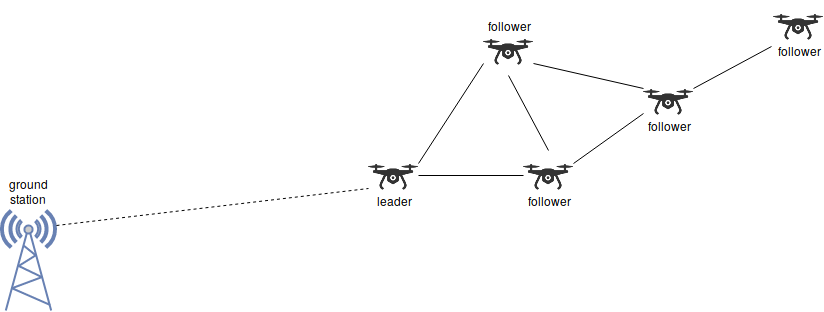
\includegraphics[scale=0.5]{Pictures/staticLeader.png}
	\caption{Static Leader Architecture}
	\label{fig: staticLeader}
	\captionsetup{font={footnotesize,bf,it}}
\end{figure}

The linux machine on the leader runs the \textit{serialros} node, as described in the last section. The \textit{serialros} node is also run on the ground station. This allows transfer of specified ros topics and services between the leader and the ground station. And since, the leader has access to all the ros topics and services of all the UAVs, sepcifying these topics in the \textit{serialros} configuration file would send these topics to the ground station, in the downlink. Typically, the ground station would not need to send any topics to the UAVs, in the uplink. It may need to access some ros services of the UAVs. This can be done by specifying these remote services in the configuration file of \textit{serialros}, at the ground station.

Thus, \textit{Static Leader} architecture combines both long range and short range communication aspects. While the wifi mesh network enables communication among the UAVs for robust distributed applications, the leader established long range communication with the ground station. One of the advantages of this architecture is that the long range radios are only needed at the leader. Also note that, since there are only two long range radios operating, one at the ground station and one on the leader, we can use RFDs, in peer to peer configuration, which offers best performance than either of the point to multipoint firmwares.

However, as mentioned earlier, this architecture assumes that all the UAVs are always connected via the mesh network, which may turn out be false. Moreover, since there is only one leader, there is a single point of failure in the system. In a case where the leader fails, for whatever reason, the ground station link would be gone. The need for addressing these issues brings us to the next section, \textit{Dynamic Leader}

\subsection{Dynamic Leader}
In \textit{Dynamic Leader} architecture, all the UAVs are mounted with RFDs. The RFDs are configured in asynchronous point to multipoint firmware, instead of the default peer to peer firmware. Unlike the \textit{Static Leader} architecture, we do not designate any UAV as a leader in this architecture. We have written a set of ROS nodes, complementing the \textit{serialros} package, which will set the leader dynamically. Let us now, briefly get an overview of this system.

We define three modes for all the UAVs in this architecture; \textit{leader}, \textit{follower} and \textit{emergency}. Except at the time of initiatialization, every UAV has to be in one of these three modes, at any given time, for the entire duration. During operation, at any instant, there is supposed to be only one \textit{leader}, and the remaining UAVs would be \textit{followers}. The third mode, \textit{emergency} is meant for those UAVs, which may have gotten disconnected with the mesh network.

\begin{figure}[h]
	\centering
	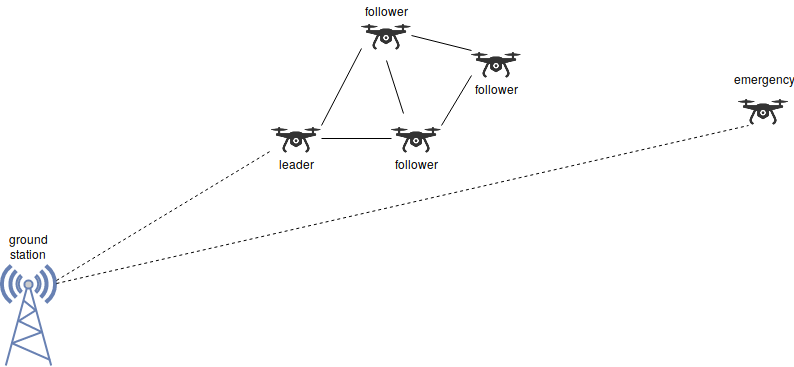
\includegraphics[scale=0.5]{Pictures/dynamicLeader.png}
	\caption{Dynamic Leader Architecture}
	\label{fig: dynamicLeader}
	\captionsetup{font={footnotesize,bf,it}}
\end{figure}

\subsubsection{link\_status}
Our aim was to design a robust system, where there is no single point of failure. Similar to the \textit{Static Leader} architecture, at any given moment, only the leader \textit{leader} sends the data to the ground station, on behalf of all the UAVs. If any of the UAVs gets disconnected from the wifi mesh network, it detects that it is not in the mesh anymore and goes into \textit{emergency} mode. While in \textit{emergency} mode, the UAV sends its data itself to the ground station. The functionality of checking if the UAV is in the mesh network or not is implement in the ROS node \textit{link\_status.py}.

\subsubsection{get\_leader service}
Apart from the \textit{leader}, one of the UAVs is designated as a \textit{standby leader}. Every UAV in the mesh network periodically seeks the \textit{leader} in the network. If there is a current \textit{leader} in the network, it would respond with its id. If there is no response and the request is timed out, the current \textit{standby leader} becomes the new \textit{leader}. This functionality of seeking the leader and the leader responding is implemented in the ROS service \textit{get\_leader.py}.

\subsubsection{uav.py}
Note that any of the UAVs may go into the \textit{emergency} mode and start transmitting data to the ground station. To allow this, RFDs are mounted on all the UAVs, powered on, ready to send the data. But, to send and receive ros topics and access ros servies via the RFD, the host machines need to the use the \textit{serialros package} as described earlier. While in \textit{leader} mode, the UAVs transmit data to the ground staion, they would not transmit anything while in \textit{follower} mode, and they would, again transmit data if they go into \textit{emergency} mode. Furthermore, they have to send ros topics of all the UAVs while they are in \textit{leader} mode, while they would send only their ros topics when they are \textit{emergency} mode.

\begin{figure}[h]
	\centering
	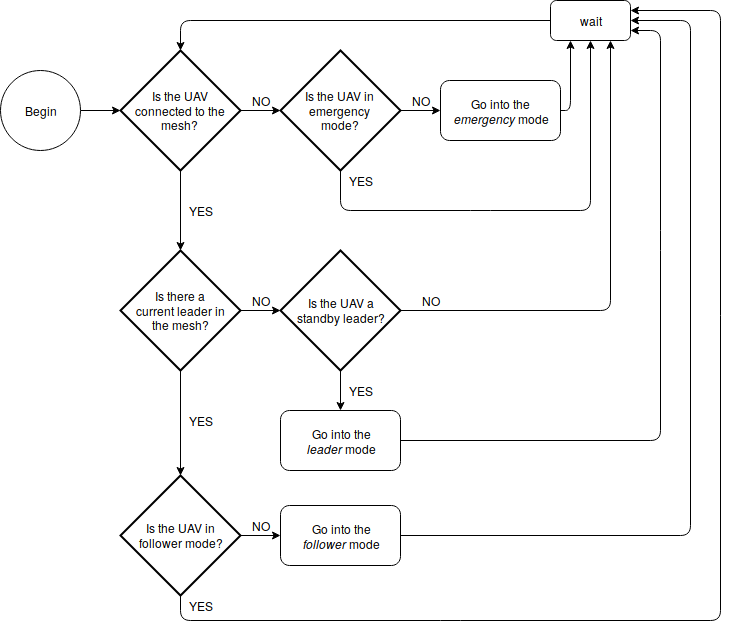
\includegraphics[scale=0.6]{Pictures/modeFlowChart.png}
	\caption{Flowchart depicting changing mode of a UAV}
	\label{fig: modeFlowChart}
	\captionsetup{font={footnotesize,bf,it}}
\end{figure}

All the above functionality requires launching and terminating the \textit{serialros} node arbitrarily. Moreover, the \textit{serialros} node needs to be launched with a different configuration file in each mode, specifying different ros topics and services in the configuration file. To achieve this functionality, we have written a ROS node, \textit{uav.py}, which, using the earlier mentioned nodes \textit{link\_status.py} and \textit{get\_leader.py}, keeps launching and terminating the \textit{serialros} node with a configuration file depending the current mode of the UAV. Figure \ref{fig: modeFlowChart} shows a flowchart depicting the changing mode of a UAV.

All the three ros nodes described above have been written as ROS package, \textit{swarmBaba}. As mentioned, the \textit{uav.py} node uses \textit{serialros} node for sending and receiving topics via the RFD. Thus, this package \textit{swarmBaba} is not independent and \textit{serialros} is a prerequisit for using it. The source code and instructions on how to use it can found at \url{https://github.com/saiadityachundi/swarmBaba}.

\subsubsection{RFD configuration}
Note that in the downlink, all the UAVs which have to transmit to the ground station would have their DESTID parameter set as 1, assuming the RFD at the ground station has its NODEID set as 1. However, for the uplink, the RFD at the ground station sets its DESTID as 65535, configuring the RFD in broadcast mode. No ros topics are sent in the uplink. The uplink is used for accessing ros services offered by the UAVs. Typically, the ground station rarely uses these services. Thus, the long range communication link between the UAVs and the ground station sees much higher data on the downlink than the uplink.

In the \textit{Dynamic Leader} architecture, only the \textit{leader} would transmit data to the ground station, when all the UAVs are in the network. A UAV which disconnected from the mesh network, would have to transmit data to the ground station. However, that does not often. It is safe to assume that in this architecture, there are not many radios transmitting to the ground station. Thus, using asynchronous firmware for the RFDs makes more sense than the synchronous firmware, because much of the bandwidth would be wasted in the latter case, where not all of the radios are transmitting data.



